% Generated by Sphinx.
\def\sphinxdocclass{report}
\documentclass[letterpaper,10pt,english]{sphinxmanual}
\usepackage[utf8]{inputenc}
\DeclareUnicodeCharacter{00A0}{\nobreakspace}
\usepackage{cmap}
\usepackage[T1]{fontenc}
\usepackage{babel}
\usepackage{times}
\usepackage[Bjarne]{fncychap}
\usepackage{longtable}
\usepackage{sphinx}
\usepackage{multirow}


\title{Zelig Documentation}
\date{May 12, 2014}
\release{5.0}
\author{The Zelig Team}
\newcommand{\sphinxlogo}{}
\renewcommand{\releasename}{Release}
\makeindex

\makeatletter
\def\PYG@reset{\let\PYG@it=\relax \let\PYG@bf=\relax%
    \let\PYG@ul=\relax \let\PYG@tc=\relax%
    \let\PYG@bc=\relax \let\PYG@ff=\relax}
\def\PYG@tok#1{\csname PYG@tok@#1\endcsname}
\def\PYG@toks#1+{\ifx\relax#1\empty\else%
    \PYG@tok{#1}\expandafter\PYG@toks\fi}
\def\PYG@do#1{\PYG@bc{\PYG@tc{\PYG@ul{%
    \PYG@it{\PYG@bf{\PYG@ff{#1}}}}}}}
\def\PYG#1#2{\PYG@reset\PYG@toks#1+\relax+\PYG@do{#2}}

\expandafter\def\csname PYG@tok@gd\endcsname{\def\PYG@tc##1{\textcolor[rgb]{0.63,0.00,0.00}{##1}}}
\expandafter\def\csname PYG@tok@gu\endcsname{\let\PYG@bf=\textbf\def\PYG@tc##1{\textcolor[rgb]{0.50,0.00,0.50}{##1}}}
\expandafter\def\csname PYG@tok@gt\endcsname{\def\PYG@tc##1{\textcolor[rgb]{0.00,0.27,0.87}{##1}}}
\expandafter\def\csname PYG@tok@gs\endcsname{\let\PYG@bf=\textbf}
\expandafter\def\csname PYG@tok@gr\endcsname{\def\PYG@tc##1{\textcolor[rgb]{1.00,0.00,0.00}{##1}}}
\expandafter\def\csname PYG@tok@cm\endcsname{\let\PYG@it=\textit\def\PYG@tc##1{\textcolor[rgb]{0.25,0.50,0.56}{##1}}}
\expandafter\def\csname PYG@tok@vg\endcsname{\def\PYG@tc##1{\textcolor[rgb]{0.73,0.38,0.84}{##1}}}
\expandafter\def\csname PYG@tok@m\endcsname{\def\PYG@tc##1{\textcolor[rgb]{0.13,0.50,0.31}{##1}}}
\expandafter\def\csname PYG@tok@mh\endcsname{\def\PYG@tc##1{\textcolor[rgb]{0.13,0.50,0.31}{##1}}}
\expandafter\def\csname PYG@tok@cs\endcsname{\def\PYG@tc##1{\textcolor[rgb]{0.25,0.50,0.56}{##1}}\def\PYG@bc##1{\setlength{\fboxsep}{0pt}\colorbox[rgb]{1.00,0.94,0.94}{\strut ##1}}}
\expandafter\def\csname PYG@tok@ge\endcsname{\let\PYG@it=\textit}
\expandafter\def\csname PYG@tok@vc\endcsname{\def\PYG@tc##1{\textcolor[rgb]{0.73,0.38,0.84}{##1}}}
\expandafter\def\csname PYG@tok@il\endcsname{\def\PYG@tc##1{\textcolor[rgb]{0.13,0.50,0.31}{##1}}}
\expandafter\def\csname PYG@tok@go\endcsname{\def\PYG@tc##1{\textcolor[rgb]{0.20,0.20,0.20}{##1}}}
\expandafter\def\csname PYG@tok@cp\endcsname{\def\PYG@tc##1{\textcolor[rgb]{0.00,0.44,0.13}{##1}}}
\expandafter\def\csname PYG@tok@gi\endcsname{\def\PYG@tc##1{\textcolor[rgb]{0.00,0.63,0.00}{##1}}}
\expandafter\def\csname PYG@tok@gh\endcsname{\let\PYG@bf=\textbf\def\PYG@tc##1{\textcolor[rgb]{0.00,0.00,0.50}{##1}}}
\expandafter\def\csname PYG@tok@ni\endcsname{\let\PYG@bf=\textbf\def\PYG@tc##1{\textcolor[rgb]{0.84,0.33,0.22}{##1}}}
\expandafter\def\csname PYG@tok@nl\endcsname{\let\PYG@bf=\textbf\def\PYG@tc##1{\textcolor[rgb]{0.00,0.13,0.44}{##1}}}
\expandafter\def\csname PYG@tok@nn\endcsname{\let\PYG@bf=\textbf\def\PYG@tc##1{\textcolor[rgb]{0.05,0.52,0.71}{##1}}}
\expandafter\def\csname PYG@tok@no\endcsname{\def\PYG@tc##1{\textcolor[rgb]{0.38,0.68,0.84}{##1}}}
\expandafter\def\csname PYG@tok@na\endcsname{\def\PYG@tc##1{\textcolor[rgb]{0.25,0.44,0.63}{##1}}}
\expandafter\def\csname PYG@tok@nb\endcsname{\def\PYG@tc##1{\textcolor[rgb]{0.00,0.44,0.13}{##1}}}
\expandafter\def\csname PYG@tok@nc\endcsname{\let\PYG@bf=\textbf\def\PYG@tc##1{\textcolor[rgb]{0.05,0.52,0.71}{##1}}}
\expandafter\def\csname PYG@tok@nd\endcsname{\let\PYG@bf=\textbf\def\PYG@tc##1{\textcolor[rgb]{0.33,0.33,0.33}{##1}}}
\expandafter\def\csname PYG@tok@ne\endcsname{\def\PYG@tc##1{\textcolor[rgb]{0.00,0.44,0.13}{##1}}}
\expandafter\def\csname PYG@tok@nf\endcsname{\def\PYG@tc##1{\textcolor[rgb]{0.02,0.16,0.49}{##1}}}
\expandafter\def\csname PYG@tok@si\endcsname{\let\PYG@it=\textit\def\PYG@tc##1{\textcolor[rgb]{0.44,0.63,0.82}{##1}}}
\expandafter\def\csname PYG@tok@s2\endcsname{\def\PYG@tc##1{\textcolor[rgb]{0.25,0.44,0.63}{##1}}}
\expandafter\def\csname PYG@tok@vi\endcsname{\def\PYG@tc##1{\textcolor[rgb]{0.73,0.38,0.84}{##1}}}
\expandafter\def\csname PYG@tok@nt\endcsname{\let\PYG@bf=\textbf\def\PYG@tc##1{\textcolor[rgb]{0.02,0.16,0.45}{##1}}}
\expandafter\def\csname PYG@tok@nv\endcsname{\def\PYG@tc##1{\textcolor[rgb]{0.73,0.38,0.84}{##1}}}
\expandafter\def\csname PYG@tok@s1\endcsname{\def\PYG@tc##1{\textcolor[rgb]{0.25,0.44,0.63}{##1}}}
\expandafter\def\csname PYG@tok@gp\endcsname{\let\PYG@bf=\textbf\def\PYG@tc##1{\textcolor[rgb]{0.78,0.36,0.04}{##1}}}
\expandafter\def\csname PYG@tok@sh\endcsname{\def\PYG@tc##1{\textcolor[rgb]{0.25,0.44,0.63}{##1}}}
\expandafter\def\csname PYG@tok@ow\endcsname{\let\PYG@bf=\textbf\def\PYG@tc##1{\textcolor[rgb]{0.00,0.44,0.13}{##1}}}
\expandafter\def\csname PYG@tok@sx\endcsname{\def\PYG@tc##1{\textcolor[rgb]{0.78,0.36,0.04}{##1}}}
\expandafter\def\csname PYG@tok@bp\endcsname{\def\PYG@tc##1{\textcolor[rgb]{0.00,0.44,0.13}{##1}}}
\expandafter\def\csname PYG@tok@c1\endcsname{\let\PYG@it=\textit\def\PYG@tc##1{\textcolor[rgb]{0.25,0.50,0.56}{##1}}}
\expandafter\def\csname PYG@tok@kc\endcsname{\let\PYG@bf=\textbf\def\PYG@tc##1{\textcolor[rgb]{0.00,0.44,0.13}{##1}}}
\expandafter\def\csname PYG@tok@c\endcsname{\let\PYG@it=\textit\def\PYG@tc##1{\textcolor[rgb]{0.25,0.50,0.56}{##1}}}
\expandafter\def\csname PYG@tok@mf\endcsname{\def\PYG@tc##1{\textcolor[rgb]{0.13,0.50,0.31}{##1}}}
\expandafter\def\csname PYG@tok@err\endcsname{\def\PYG@bc##1{\setlength{\fboxsep}{0pt}\fcolorbox[rgb]{1.00,0.00,0.00}{1,1,1}{\strut ##1}}}
\expandafter\def\csname PYG@tok@kd\endcsname{\let\PYG@bf=\textbf\def\PYG@tc##1{\textcolor[rgb]{0.00,0.44,0.13}{##1}}}
\expandafter\def\csname PYG@tok@ss\endcsname{\def\PYG@tc##1{\textcolor[rgb]{0.32,0.47,0.09}{##1}}}
\expandafter\def\csname PYG@tok@sr\endcsname{\def\PYG@tc##1{\textcolor[rgb]{0.14,0.33,0.53}{##1}}}
\expandafter\def\csname PYG@tok@mo\endcsname{\def\PYG@tc##1{\textcolor[rgb]{0.13,0.50,0.31}{##1}}}
\expandafter\def\csname PYG@tok@mi\endcsname{\def\PYG@tc##1{\textcolor[rgb]{0.13,0.50,0.31}{##1}}}
\expandafter\def\csname PYG@tok@kn\endcsname{\let\PYG@bf=\textbf\def\PYG@tc##1{\textcolor[rgb]{0.00,0.44,0.13}{##1}}}
\expandafter\def\csname PYG@tok@o\endcsname{\def\PYG@tc##1{\textcolor[rgb]{0.40,0.40,0.40}{##1}}}
\expandafter\def\csname PYG@tok@kr\endcsname{\let\PYG@bf=\textbf\def\PYG@tc##1{\textcolor[rgb]{0.00,0.44,0.13}{##1}}}
\expandafter\def\csname PYG@tok@s\endcsname{\def\PYG@tc##1{\textcolor[rgb]{0.25,0.44,0.63}{##1}}}
\expandafter\def\csname PYG@tok@kp\endcsname{\def\PYG@tc##1{\textcolor[rgb]{0.00,0.44,0.13}{##1}}}
\expandafter\def\csname PYG@tok@w\endcsname{\def\PYG@tc##1{\textcolor[rgb]{0.73,0.73,0.73}{##1}}}
\expandafter\def\csname PYG@tok@kt\endcsname{\def\PYG@tc##1{\textcolor[rgb]{0.56,0.13,0.00}{##1}}}
\expandafter\def\csname PYG@tok@sc\endcsname{\def\PYG@tc##1{\textcolor[rgb]{0.25,0.44,0.63}{##1}}}
\expandafter\def\csname PYG@tok@sb\endcsname{\def\PYG@tc##1{\textcolor[rgb]{0.25,0.44,0.63}{##1}}}
\expandafter\def\csname PYG@tok@k\endcsname{\let\PYG@bf=\textbf\def\PYG@tc##1{\textcolor[rgb]{0.00,0.44,0.13}{##1}}}
\expandafter\def\csname PYG@tok@se\endcsname{\let\PYG@bf=\textbf\def\PYG@tc##1{\textcolor[rgb]{0.25,0.44,0.63}{##1}}}
\expandafter\def\csname PYG@tok@sd\endcsname{\let\PYG@it=\textit\def\PYG@tc##1{\textcolor[rgb]{0.25,0.44,0.63}{##1}}}

\def\PYGZbs{\char`\\}
\def\PYGZus{\char`\_}
\def\PYGZob{\char`\{}
\def\PYGZcb{\char`\}}
\def\PYGZca{\char`\^}
\def\PYGZam{\char`\&}
\def\PYGZlt{\char`\<}
\def\PYGZgt{\char`\>}
\def\PYGZsh{\char`\#}
\def\PYGZpc{\char`\%}
\def\PYGZdl{\char`\$}
\def\PYGZhy{\char`\-}
\def\PYGZsq{\char`\'}
\def\PYGZdq{\char`\"}
\def\PYGZti{\char`\~}
% for compatibility with earlier versions
\def\PYGZat{@}
\def\PYGZlb{[}
\def\PYGZrb{]}
\makeatother

\begin{document}

\maketitle
\tableofcontents
\phantomsection\label{index::doc}


Contents:


\chapter{Introduction}
\label{1_introduction:introduction}\label{1_introduction:welcome-to-zelig-s-documentation}\label{1_introduction::doc}

\section{What Zelig and R do}
\label{1_introduction:what-zelig-and-r-do}
Zelig \footnote{
Zelig is named after a Woody Allen movie about a man who had the strange ability to become the physical reflection of anyone he met --- Scottish, African-American, Indian, Chinese, thin, obese, medical doctor, Hassidic rabbi, anything --- and thus to fit well in any situation.
} is an easy-to-use program that can estimate and help interpret the results of an enormous and growing range of statistical models. It literally is “everyone’s statistical software” because Zelig’s unified framework incorporates everyone else’s (R) code. We also hope it will become “everyone’s statistical software” for applications, and we have designed Zelig so that anyone can use it or add their models to it.

When you are using Zelig, you are also using R, a powerful statistical software language. You do not need to learn R separately, however, since this manual introduces you to R through Zelig, which simplifies R and reduces the amount of programming knowledge you need to get started. Because so many individuals contribute different packages to R (each with their own syntax and documentation), estimating a statistical model can be a frustrating experience. Users need to know which package contains the model, find the modeling command within the package, and refer to the manual page for the model-specific arguments. In contrast, Zelig users can skip these start-up costs and move directly to data analyses. Using Zelig’s unified command syntax, you gain the convenience of a packaged program, without losing any of the power of R’s underlying statistical procedures.

In addition to generalizing R packages and making existing methods easier to use, Zelig includes infrastructure that can improve all existing methods and R programs. Even if you know R, using Zelig greatly simplifies your work. It mimics the popular Clarify program for Stata (and thus the suggestions of King, Tomz, and Wittenberg, 2000) by translating the raw output of existing statistical procedures into quantities that are of direct interest to researchers. Instead of trying to interpret coefficients parameterized for modeling convenience, Zelig makes it easy to compute quantities of real interest: probabilities, predicted values, expected values, first differences, and risk ratios, along with confidence intervals, standard errors, or full posterior (or sampling) densities for all quantities. Zelig extends Clarify by seamlessly integrating an option for bootstrapping into the simulation of quantities of interest. It also integrates a full suite of nonparametric matching methods as a preprocessing step to improve the performance of any parametric model for causal inference (see MatchIt). For missing data, Zelig accepts multiply imputed datasets created by Amelia (see King, Honaker, Joseph, and Scheve, 2001) and other programs, allowing users to analyze them as if they were a single, fully observed dataset. Zelig outputs replication data sets so that you (and if you wish, anyone else) will always be able to replicate the results of your analyses (see King, 1995). Several powerful Zelig commands also make running multiple analyses and recoding variables simple.

Using R in combination with Zelig has several advantages over commercial statistical software. R and Zelig are part of the open source movement, which is roughly based on the principles of science. That is, anyone who adds functionality to open source software or wishes to redistribute it (legally) must provide the software accompanied by its source free of charge.As specified in the {[}\href{http://www.gnu.org/copyleft}{http://www.gnu.org/copyleft}/\textbar{}\textbar{}GNU General Public License{]}. If you find a bug in open source software and post a note to the appropriate mailing list, a solution you can use will likely be posted quickly by one of the thousands of people using the program all over the world. Since you can see the source code, you might even be able to fix it yourself. In contrast, if something goes wrong with commercial software, you have to wait for the programmers at the company to fix it (and speaking with them is probably out of the question), and wait for a new version to be released.

We find that Zelig makes students and colleagues more amenable to using R, since the startup costs are lower, and since the manual and software are relatively self-contained. This manual even includes an appendix devoted to the basics of advanced R programming, although you will not need it to run most procedures in Zelig. A large and growing fraction of the world's quantitative methodologists and statisticians are moving to R, and the base of programs available for R is quickly surpassing all alternatives. In addition to built-in functions, R is a complete programming language, which allows you to design new functions to suit your needs. R has the dual advantage that you do not need to understand how to program to use it, but if it turns out that you want to do something more complicated, you do not need to learn another program. In addition, methodologists all over the world add new functions all the time, so if the function you need wasn't there yesterday, it may be available today.


\section{Getting Help}
\label{1_introduction:getting-help}
You may find documentation for Zelig on-line (and hence must be on-line to access it). If you are unable to connect to the Internet, we recommend that you print the pdf version of this document for your reference.

If you are on-line, you may access comprehensive help files for Zelig commands and for each of the models. For example, load the Zelig library and then type at the R prompt:

\begin{Verbatim}[commandchars=\\\{\}]
help.zelig\PYG{p}{(}command\PYG{p}{)}  \PYG{c+c1}{\PYGZsh{} For help with all zelig commands.}
help.zelig\PYG{p}{(}logit\PYG{p}{)}  \PYG{c+c1}{\PYGZsh{} For help with the logit model.}
\end{Verbatim}

In addition, help.zelig() searches the manual pages for R in addition to the Zelig specific pages. On certain rare occasions, the name of the help topic in Zelig and in R are identical. In these cases, help.zelig() will return the Zelig help page by default. If you wish to access the R help page, you should use help(topic).

In addition, built-in examples with sample data and plots are available for each model. For example, type demo(logit) to view the demo for the logit model. Commented code for each model is available under the examples section of each model reference page.

Please direct inquiries and problems about Zelig to our listserv at \href{mailto:zelig@lists.gking.harvard.edu}{zelig@lists.gking.harvard.edu}. We suggest you subscribe to this mailing list while learning and using Zelig: go to \href{https://lists.gking.harvard.edu/mailman/listinfo/zelig}{https://lists.gking.harvard.edu/mailman/listinfo/zelig}. (You can choose to receive email in digest form, so that you will never receive more than one message per day.) You can also browse or search our {[}\href{https://lists.gking.harvard.edu/pipermail/zelig}{https://lists.gking.harvard.edu/pipermail/zelig}/\textbar{}\textbar{}archive{]} of previous messages before posting your query.


\section{How to Cite Zelig}
\label{1_introduction:how-to-cite-zelig}
To cite Zelig as a whole, please reference these two sources:
\begin{itemize}
\item {} 
Kosuke Imai, Gary King, and Olivia Lau. 2007. ``Zelig: Everyone's Statistical Software'', \href{http://GKing.harvard.edu/zelig}{http://GKing.harvard.edu/zelig}.

\item {} 
Imai, Kosuke, Gary King, and Olivia Lau. (2008). “Toward A Common Framework for Statistical Analysis and Development.” Journal of Computational and Graphical Statistics, Vol. 17, No. 4 (December), pp. 892-913.

\end{itemize}

To refer to a particular Zelig model, please refer to the “how to cite” portion at the end of each model documentation section.

\begin{Verbatim}[commandchars=\\\{\}]
x \PYG{o}{\PYGZlt{}\PYGZhy{}} \PYG{l+m}{1}\PYG{o}{:}\PYG{l+m}{10}
y \PYG{o}{\PYGZlt{}\PYGZhy{}} rnorm\PYG{p}{(}\PYG{l+m}{10}\PYG{p}{)}
plot\PYG{p}{(}x\PYG{p}{,} y\PYG{p}{)}
\end{Verbatim}
\begin{figure}[htbp]
\centering
\capstart


\includegraphics{unnamed-chunk-2.png}
\caption{plot of chunk unnamed-chunk-2}\end{figure}

\begin{Verbatim}[commandchars=\\\{\}]
print\PYG{p}{(}y\PYG{p}{)}
\end{Verbatim}

\begin{Verbatim}[commandchars=\\\{\}]
\PYG{c}{\PYGZsh{}\PYGZsh{}  [1]  0.56612  1.38396  0.02811  1.88444 \PYGZhy{}0.65357  0.79660  0.72366}
\PYG{c}{\PYGZsh{}\PYGZsh{}  [8]  0.24537  1.92806  0.44184}
\end{Verbatim}

\begin{Verbatim}[commandchars=\\\{\}]
\PYG{l+m}{2} \PYG{o}{+} \PYG{l+m}{3}
\end{Verbatim}

\begin{Verbatim}[commandchars=\\\{\}]
\PYG{c}{\PYGZsh{}\PYGZsh{} [1] 5}
\end{Verbatim}


\chapter{Installation}
\label{2_install:installation}\label{2_install::doc}
To use Zelig, you must install the statistical program R (if it is not already installed), the Zelig package, and some R libraries (coda, MCMCpack, sandwich, VGAM, and zoo).

Note: In this document, \textgreater{} denotes the R prompt.


\section{If You Are New to R}
\label{2_install:if-you-are-new-to-r}
If you are new to R, we recommend that you read the following section on installation procedures as well as the overview of R syntax and usage in Sref\{a:R\}.

This distribution works on a variety of platforms, including Windows (see Section {[}ss:win{]}), MacOSX (see Section {[}ss:osx{]}), and Linux (see Section {[}ss:unix{]}). Alternatively, you may access R from your PC using a terminal window or an X-windows tunnel to a Linux or Unix server (see Section {[}ss:unix{]}). Most servers have R installed; if not, contact your network administrator.

There are advantages and disadvantages to each type of installation. On a personal computer, R is easier to install and launch. Using R remotely on a server requires a bit more set-up, but does not tie up your local CPU, and allows you to take advantage of the server's speed.


\section{If You Know R}
\label{2_install:if-you-know-r}
We recommend that you launch R and type

\begin{Verbatim}[commandchars=\\\{\}]
install.packages\PYG{p}{(}\PYG{l+s}{\PYGZdq{}}\PYG{l+s}{Zelig\PYGZdq{}}\PYG{p}{)}
\end{Verbatim}

then proceed to ??Sref\{overview\}??. For Windows R, you may edit the Rprofile file to load Zelig automatically at launch (after which you will no longer need to type library(Zelig) at startup). Simply add the line:

\begin{Verbatim}[commandchars=\\\{\}]
options\PYG{p}{(}defaultPackages \PYG{o}{=} c\PYG{p}{(}getOption\PYG{p}{(}\PYG{l+s}{\PYGZdq{}}\PYG{l+s}{defaultPackages\PYGZdq{}}\PYG{p}{)}\PYG{p}{,} \PYG{l+s}{\PYGZdq{}}\PYG{l+s}{Zelig\PYGZdq{}}\PYG{p}{)}\PYG{p}{)}
\end{Verbatim}


\section{Windows}
\label{2_install:windows}

\subsection{Installing R}
\label{2_install:installing-r}
Go to the Comprehensive R Archive Network website (\href{http://www.r-project.org}{http://www.r-project.org}) and download the latest \href{http://cran.us.r-project.org/bin/windows/base/}{installer} for Windows at \href{http://cran.us.r-project.org/bin/windows/base/}{http://cran.us.r-project.org/bin/windows/base/} Double-click the .exe file to launch the R installer. We recommend that you accept the default installation options if this your first installation.

Installing Zelig

Once R is installed, you must install the Zelig package:

\begin{Verbatim}[commandchars=\\\{\}]
install.packages\PYG{p}{(}\PYG{l+s}{\PYGZdq{}}\PYG{l+s}{Zelig\PYGZdq{}}\PYG{p}{)}
\end{Verbatim}

Zelig will load the optional libraries whenever their functions are needed; it is not necessary to load any package other than Zelig at startup.
\begin{enumerate}
\item {} 
Alternatively, you may use the drop down menus to install Zelig.

\end{enumerate}
\begin{enumerate}
\item {} 
Download the latest release of Zelig from \href{http://cran.r-project.org/web/packages/Zelig/index.html}{CRAN}. Store the .zip files in your R program directory. For example, the default R program directory is C:Program FilesRR-rvers.Note that when updating R to the latest release, the installer does not delete previous versions from your C:Program FilesRdirectory. In this example, the subdirectory R-rversstores R version fullvers. Thus, if you have a different version of R installed, you should change the last part of the R program directory file path accordingly.

\item {} 
Start R. From the drop-down menus, select the “Packages” menu and then the “Install Files from Local Zip Files” option.

\item {} 
A window will pop up, allowing you to select one of the downloaded files for installation. There is no need to unzip the files prior to installation. Repeat and select the other downloaded file for installation.

\item {} 
At the R prompt, type library(Zelig) to load the functionality described in this manual. Note that Zelig will automatically load the other libraries as necessary.

\item {} 
An additional recommended but optional step is to set up R to load Zelig automatically at launch. (If you skip this step, you must type library(Zelig) at the beginning of every R session.) To automate this process, edit the Rprofile file located in the R program subdirectory (in our example). Using a text editor such as Windows notepad, add the following line to the Rprofile file:

\end{enumerate}

\begin{Verbatim}[commandchars=\\\{\}]
options\PYG{p}{(}defaultPackages \PYG{o}{=} c\PYG{p}{(}getOption\PYG{p}{(}\PYG{l+s}{\PYGZdq{}}\PYG{l+s}{defaultPackages\PYGZdq{}}\PYG{p}{)}\PYG{p}{,} \PYG{l+s}{\PYGZdq{}}\PYG{l+s}{Zelig\PYGZdq{}}\PYG{p}{)}\PYG{p}{)}
\end{Verbatim}

Zelig is distributed under the \href{http://www.gnu.org/licenses/gpl.txt}{GNU General Public License}. After installation, the source code is located in your R library directory, which is by default C:Program FilesRR-rverslibraryZelig.


\subsection{Updating Zelig}
\label{2_install:updating-zelig}
There are two ways to update Zelig.
\begin{enumerate}
\item {} 
We recommend that you periodically update Zelig at the R prompt by typing:

\end{enumerate}

\begin{Verbatim}[commandchars=\\\{\}]
update.packages\PYG{p}{(}\PYG{p}{)}
\end{Verbatim}
\begin{enumerate}
\setcounter{enumi}{1}
\item {} 
Alternatively, you may use the procedure outlined in {[}win.zelig{]} to periodically update Zelig. Simply download the latest .zip file and follow the steps.

\end{enumerate}


\section{Mac OS X}
\label{2_install:mac-os-x}

\subsection{Installing R}
\label{2_install:id1}
If you are using MacOS X, you may install the latest version of R (fullvers at this time) from the CRAN website \href{http://cran.us.r-project.org/bin/macosx/}{http://cran.us.r-project.org/bin/macosx/}.


\subsection{Installing Zelig}
\label{2_install:installing-zelig}
Once R is installed, you must install the Zelig package:

\begin{Verbatim}[commandchars=\\\{\}]
install.packages\PYG{p}{(}\PYG{l+s}{\PYGZdq{}}\PYG{l+s}{Zelig\PYGZdq{}}\PYG{p}{)}
\end{Verbatim}

Alternatively, you may use the drop down menus to install Zelig.
\begin{enumerate}
\item {} 
Download the latest release of Zelig from \href{http://cran.us.r-project.org/bin/windows/base/}{CRAN}. Save the .tgz files in a convenient place.

\item {} 
Start R. From the drop-down menus, select the “Packages” menu and then the “Install Files from Local Files” option.

\item {} 
A window will pop up, allowing you to select the downloaded file for installation. There is no need to unzip the file prior to installation.

\end{enumerate}


\section{Version Compatibility}
\label{2_install:version-compatibility}
In addition to R itself, Zelig also depends on several R packages maintained by other development teams. Although we make every effort to keep the latest version of Zelig up-to-date with the latest version of those packages, there may occasionally be incompatibilities. See {[}table.compat{]} in the Appendix for a list of packages tested to be compatibile with a given Zelig release. You may obtain older versions of most packages at \href{http://www.r-project.org}{http://www.r-project.org}.


\section{UNIX and Linux}
\label{2_install:unix-and-linux}

\subsection{Installing R}
\label{2_install:id3}
Type R at the terminal prompt (which we denote as \% in this section) to see if R is available. (Typing q() will enable you to quit.) If it is installed, proceed to the next section. If it is not installed and you are not the administrator, contact that individual, kindly request that they install R on the server, and continue to the next section. If you have administrator privileges, you may download the latest release at the \href{http://cran.r-project.org/}{CRAN} website. Although installation varies according to your Linux distribution, we provide an example for Red Hat Linux 9.0 as a guide.
\begin{enumerate}
\item {} 
Log in as root.

\item {} 
Download the appropriate binary file for Red Hat 9 from CRAN.

\item {} 
Type the following command at the terminal prompt:

\end{enumerate}


\subsection{Installing Zelig}
\label{2_install:id5}
Before installing Zelig, you need to create a local R library directory. If you have done so already, you can skip to Section {[}unix.zelig{]}. If not, you must do so before proceeding because most users do not have authorization to install programs globally. Suppose we want the directory to be \textasciitilde{}/.R/library. At the terminal prompt in your home directory, type:

\begin{Verbatim}[commandchars=\\\{\}]
mkdir \PYGZti{}/.R \PYGZti{}/.R/library
\end{Verbatim}

Now you are ready to install Zelig.

There are two ways to proceed.
\begin{enumerate}
\item {} 
Recommended procedure:

\end{enumerate}
\begin{enumerate}
\item {} 
Open the \textasciitilde{}/.Renviron file (or create it if it does not exist) and add the following line:

\end{enumerate}
\begin{quote}

RLIBS = '' /.R/library''
\end{quote}

You only need to perform this step once.
\begin{enumerate}
\item {} 
Start R. At the R prompt, type:

\end{enumerate}

\begin{Verbatim}[commandchars=\\\{\}]
install.packages\PYG{p}{(}\PYG{l+s}{\PYGZdq{}}\PYG{l+s}{Zelig\PYGZdq{}}\PYG{p}{)}
\end{Verbatim}
\begin{enumerate}
\setcounter{enumi}{1}
\item {} 
Finally, create a .Rprofile file in your home directory, containing the line:

\end{enumerate}

\begin{Verbatim}[commandchars=\\\{\}]
library\PYG{p}{(}Zelig\PYG{p}{)}
\end{Verbatim}

This will load Zelig every time you start R.

After installation, the source code is located in your R library directory. If you followed the example above, this is  /.R/library/Zelig/.

Updating Zelig

There are two ways to update Zelig.
\begin{enumerate}
\item {} 
We recommend that you start R and, at the R prompt, type:

\end{enumerate}

\begin{Verbatim}[commandchars=\\\{\}]
update.packages\PYG{p}{(}\PYG{p}{)}
\end{Verbatim}
\begin{enumerate}
\setcounter{enumi}{1}
\item {} 
Alternatively, you may remove an old version by command by typing:

\end{enumerate}
\begin{quote}

R CMD REMOVE Zelig
\end{quote}

Now you are ready to install Zelig.


\chapter{Data Analysis Commands}
\label{3_data_analysis:data-analysis-commands}\label{3_data_analysis::doc}

\section{Command Syntax}
\label{3_data_analysis:command-syntax}
Once R is installed, you only need to know a few basic elements to get started. It's important to remember that R, like any spoken language, has rules for proper syntax. Unlike English, however, the rules for intelligible R are small in number and quite precise (see Section {[}s:syntax{]}).


\subsection{Getting Started}
\label{3_data_analysis:getting-started}\begin{enumerate}
\item {} 
To start R under Linux or Unix, type R at the terminal prompt or M-x R under ESS.

\item {} 
The R prompt is \code{\textgreater{}}.

\item {} 
Type commands and hit enter to execute. (No additional characters, such as semicolons or commas, are necessary at the end of lines.)

\item {} 
To quit from R, type \code{q()} and press enter.

\item {} 
The \code{\#} character makes R ignore the rest of the line, and is used in this document to comment R code.

\item {} 
We highly recommend that you make a separate working directory or folder for each project.

\item {} 
Each R session has a workspace, or working memory, to store the objects that you create or input. These objects may be:

\end{enumerate}
\begin{enumerate}
\item {} 
values, which include numerical, integer, character, and logical values;

\item {} 
data structures made up of variables (vectors), matrices, and data frames; or

\item {} 
functions that perform the desired tasks on user-specified values or data structures.

\end{enumerate}

After starting R, you may at any time use Zelig's built-in help function to access on-line help for any command. To see help for all Zelig commands, type help.zelig(command), which will take you to the help page for all Zelig commands. For help with a specific Zelig or R command substitute the name of the command for the generic command. For example, type help.zelig(logit) to view help for the logit model.


\subsection{Details}
\label{3_data_analysis:details}
Zelig uses the syntax of R, which has several essential elements:
\begin{enumerate}
\item {} 
R is case sensitive. Zelig, the package or library, is not the same as zelig, the command.

\item {} 
R functions accept user-defined arguments: while some arguments are required, other optional arguments modify the function's default behavior. Enclose arguments in parentheses and separate multiple arguments with commas. For example, \code{print(x)} or \code{print(x, digits = 2)} prints the contents of the object x using the default number of digits or rounds to two digits to the right of the decimal point, respectively. You may nest commands as long as each has its own set of parentheses: \code{log(sqrt(5))} takes the square root of 5 and then takes the natural log.

\item {} 
The \textless{}- operator takes the output of the function on the right and saves them in the named object on the left. For example, \code{z.out \textless{}- zelig(\textbackslash{}dots)} stores the output from \code{zelig()} as the object z.out in your working memory. You may use z.out as an argument in other functions, view the output by typing z.out at the R prompt, or save z.out to a file using the procedures described in Section {\hyperref[3_data_analysis:saving-data]{Saving Data}}.

\item {} 
You may name your objects anything, within a few constraints:

\end{enumerate}
\begin{itemize}
\item {} 
You may only use letters (in upper or lower case) and periods to punctuate your variable names.

\item {} 
You may not use any special characters (aside from the period) or spaces to punctuate your variable names.

\item {} 
Names cannot begin with numbers. For example, R will not let you save an object as 1997.election but will let you save election.1997.

\end{itemize}
\begin{enumerate}
\setcounter{enumi}{4}
\item {} 
Use the \code{names()} command to see the contents of R objects, and the \$ operator to extract elements from R objects. For example:

\end{enumerate}

\begin{Verbatim}[commandchars=\\\{\}]
\PYG{c+c1}{\PYGZsh{} Run least squares regression and save the output in working memory:}
z.out \PYG{o}{\PYGZlt{}\PYGZhy{}} zelig\PYG{p}{(}y \PYG{o}{\PYGZti{}} x1 \PYG{o}{+} x2\PYG{p}{,} model \PYG{o}{=} \PYG{l+s}{\PYGZdq{}}\PYG{l+s}{ls\PYGZdq{}}\PYG{p}{,} data \PYG{o}{=} mydata\PYG{p}{)}
\PYG{c+c1}{\PYGZsh{} See what\PYGZsq{}s in the R object:}
names\PYG{p}{(}z.out\PYG{p}{)}
\PYG{c+c1}{\PYGZsh{}\PYGZsh{} [1] \PYGZsq{}coefficients\PYGZsq{} \PYGZsq{}residuals\PYGZsq{} \PYGZsq{}effects\PYGZsq{} \PYGZsq{}rank\PYGZsq{} Extract and display the}
\PYG{c+c1}{\PYGZsh{}\PYGZsh{} coefficients in z.out:}
z.out\PYG{o}{\PYGZdl{}}coefficients
\end{Verbatim}

6. a frame is a rectangular matrix with n rows and k
columns. Each column represents a variable and each row an observation. Each variable may have a different class. (See Section ??variable.classes?? for a list of classes.)
You may refer to specific variables from a data frame using, for example, \code{data\$variable}.
\begin{enumerate}
\setcounter{enumi}{6}
\item {} 
A list is a combination of different data structures. For example, \code{z.out} contains both coefficients (a vector) and data (a data frame). Use \code{names()} to view the elements available within a list, and the \code{\$} operator to refer to an element in a list.

\end{enumerate}

For a more comprehensive introduction, including ways to manipulate these data structures, please refer to Chapter {[}a:R{]}.


\subsection{Loading Data}
\label{3_data_analysis:loading-data}
Datasets in Zelig are stored in “data frames.” In this section, we explain the standard ways to load data from disk into memory, how to handle special cases, and how to verify that the data you loaded is what you think it is.

Standard Ways to Load Data

Make sure that the data file is saved in your working directory. You can check to see what your working directory is by starting R, and typing getwd(). If you wish to use a different directory as your starting directory, use setwd(``dirpath''), where ``dirpath'' is the full directory path of the directory you would like to use as your working directory.

After setting your working directory, load data using one of the following methods:
\begin{enumerate}
\item {} 
If your dataset is in a tab- or space-delimited .txt file, use read.table(``mydata.txt'')

\end{enumerate}
\begin{enumerate}
\item {} 
If your dataset is a comma separated table, use read.csv(``mydata.csv'').

\item {} 
To import SPSS, Stata, and other data files, use the foreign package, which automatically preserves field characteristics for each variable. Thus, variables classed as dates in Stata are automatically translated into values in the date class for R. For example:

\end{enumerate}

\begin{Verbatim}[commandchars=\\\{\}]
library\PYG{p}{(}foreign\PYG{p}{)}  \PYG{c+c1}{\PYGZsh{} Load the foreign package.}
stata.data \PYG{o}{\PYGZlt{}\PYGZhy{}} read.dta\PYG{p}{(}\PYG{l+s}{\PYGZdq{}}\PYG{l+s}{mydata.dta\PYGZdq{}}\PYG{p}{)}  \PYG{c+c1}{\PYGZsh{} For Stata data.}
spss.data \PYG{o}{\PYGZlt{}\PYGZhy{}} read.spss\PYG{p}{(}\PYG{l+s}{\PYGZdq{}}\PYG{l+s}{mydata.sav\PYGZdq{}}\PYG{p}{,} to.data.frame \PYG{o}{=} \PYG{k+kc}{TRUE}\PYG{p}{)}  \PYG{c+c1}{\PYGZsh{} For SPSS.}
\end{Verbatim}
\begin{enumerate}
\setcounter{enumi}{1}
\item {} 
To load data in R format, use load(``mydata.RData'').

\end{enumerate}
\begin{enumerate}
\item {} 
For sample data sets included with R packages such as Zelig, you may use the data() command, which is a shortcut for loading data from the sample data directories. Because the locations of these directories vary by installation, it is extremely difficult to locate sample data sets and use one of the three preceding methods; data() searches all of the currently used packages and loads sample data automatically. For example:

\end{enumerate}

\begin{Verbatim}[commandchars=\\\{\}]
library\PYG{p}{(}Zelig\PYG{p}{)}  \PYG{c+c1}{\PYGZsh{} Loads the Zelig library.}
data\PYG{p}{(}turnout\PYG{p}{)}  \PYG{c+c1}{\PYGZsh{} Loads the turnout data.}
\end{Verbatim}

Special Cases When Loading Data

These procedures apply to any of the above read commands:
\begin{enumerate}
\item {} 
If your file uses the first row to identify variable names, you should use the option header = TRUE to import those field names. For example,

\end{enumerate}

\begin{Verbatim}[commandchars=\\\{\}]
read.csv\PYG{p}{(}\PYG{l+s}{\PYGZdq{}}\PYG{l+s}{mydata.csv\PYGZdq{}}\PYG{p}{,} header \PYG{o}{=} \PYG{k+kc}{TRUE}\PYG{p}{)}
\end{Verbatim}

will read the words in the first row as the variable names and the subsequent rows (each with the same number of values as the first) as observations for each of those variables. If you have additional characters on the last line of the file or fewer values in one of the rows, you need to edit the file before attempting to read the data.
\begin{enumerate}
\setcounter{enumi}{1}
\item {} 
The R missing value code is NA. If this value is in your data, R will recognize your missing values as such. If you have instead used a place-holder value (such as -9) to represent missing data, you need to tell R this on loading the data:

\end{enumerate}

\begin{Verbatim}[commandchars=\\\{\}]
read.table\PYG{p}{(}\PYG{l+s}{\PYGZdq{}}\PYG{l+s}{mydata.tab\PYGZdq{}}\PYG{p}{,} header \PYG{o}{=} \PYG{k+kc}{TRUE}\PYG{p}{,} na.strings \PYG{o}{=} \PYG{l+s}{\PYGZdq{}}\PYG{l+s}{\PYGZhy{}9\PYGZdq{}}\PYG{p}{)}
\end{Verbatim}

Note: You must enclose your place holder values in quotes.
\begin{enumerate}
\setcounter{enumi}{2}
\item {} 
Unlike Windows, the file extension in R does not determine the default method for dealing with the file. For example, if your data is tab-delimited, but saved as a .sav file, read.table(``mydata.sav'') will load your data into R.

\end{enumerate}

Verifying You Loaded The Data Correctly

Whichever method you use, try the names(), dim(), and summary() commands to verify that the data was properly loaded. For example,

\begin{Verbatim}[commandchars=\\\{\}]
data \PYG{o}{\PYGZlt{}\PYGZhy{}} read.csv\PYG{p}{(}\PYG{l+s}{\PYGZdq{}}\PYG{l+s}{mydata.csv\PYGZdq{}}\PYG{p}{,} header \PYG{o}{=} \PYG{k+kc}{TRUE}\PYG{p}{)}  \PYG{c+c1}{\PYGZsh{} Read the data.}
dim\PYG{p}{(}data\PYG{p}{)}  \PYG{c+c1}{\PYGZsh{} Displays the dimensions of the data frame}
\PYG{c+c1}{\PYGZsh{}\PYGZsh{} [1] 16000 8 \PYGZsh{} in rows then columns.}
data\PYG{p}{[}\PYG{l+m}{1}\PYG{o}{:}\PYG{l+m}{10}\PYG{p}{,} \PYG{p}{]}  \PYG{c+c1}{\PYGZsh{} Display rows 1\PYGZhy{}10 and all columns.}
names\PYG{p}{(}data\PYG{p}{)}  \PYG{c+c1}{\PYGZsh{} Check the variable names.}
\PYG{c+c1}{\PYGZsh{}\PYGZsh{} [1] \PYGZsq{}V1\PYGZsq{} \PYGZsq{}V2\PYGZsq{} \PYGZsq{}V3\PYGZsq{} These values indicate that the variables weren\PYGZsq{}t named,}
\PYG{c+c1}{\PYGZsh{}\PYGZsh{} and took default values.}
names\PYG{p}{(}data\PYG{p}{)} \PYG{o}{\PYGZlt{}\PYGZhy{}} c\PYG{p}{(}\PYG{l+s}{\PYGZdq{}}\PYG{l+s}{income\PYGZdq{}}\PYG{p}{,} \PYG{l+s}{\PYGZdq{}}\PYG{l+s}{educate\PYGZdq{}}\PYG{p}{,} \PYG{l+s}{\PYGZdq{}}\PYG{l+s}{year\PYGZdq{}}\PYG{p}{)}  \PYG{c+c1}{\PYGZsh{} Assign variable names.}
summary\PYG{p}{(}data\PYG{p}{)}  \PYG{c+c1}{\PYGZsh{} Returning a summary for each variable.}
\end{Verbatim}

In this case, the summary() command will return the maximum, minimum, mean, median, first and third quartiles, as well as the number of missing values for each variable.


\subsection{Saving Data}
\label{3_data_analysis:saving-data}
Use save() to write data or any object to a file in your working directory. For example,

\begin{Verbatim}[commandchars=\\\{\}]
\PYG{c+c1}{\PYGZsh{}\PYGZsh{} Saves {}`mydata\PYGZsq{} to {}`mydata.RData\PYGZsq{} in your working directory.}
save\PYG{p}{(}mydata\PYG{p}{,} file \PYG{o}{=} \PYG{l+s}{\PYGZdq{}}\PYG{l+s}{mydata.RData\PYGZdq{}}\PYG{p}{)}
\PYG{c+c1}{\PYGZsh{}\PYGZsh{} Saves your entire workspace to the default {}`.RData\PYGZsq{} file.}
save.image\PYG{p}{(}\PYG{p}{)}
\end{Verbatim}

R will also prompt you to save your workspace when you use the q() command to quit. When you start R again, it will load the previously saved workspace. Restarting R will not, however, load previously used packages. You must remember to load Zelig at the beginning of every R session.

Alternatively, you can recall individually saved objects from .RData files using the load() command. For example,

\begin{Verbatim}[commandchars=\\\{\}]
load\PYG{p}{(}\PYG{l+s}{\PYGZdq{}}\PYG{l+s}{mydata.RData\PYGZdq{}}\PYG{p}{)}
\end{Verbatim}

loads the objects saved in the mydata.RData file. You may save a data frame, a data frame and associated functions, or other R objects to file.


\section{Variables}
\label{3_data_analysis:variables}

\subsection{Classes of Variables}
\label{3_data_analysis:classes-of-variables}
R variables come in several types. Certain Zelig models require dependent variables of a certain class of variable. (These are documented under the manual pages for each model.) Use class(variable) to determine the class of a variable or class(data\$variable) for a variable within a data frame.

Types of Variables

For all types of variable (vectors), you may use the c() command to “concatenate” elements into a vector, the : operator to generate a sequence of integer values, the seq() command to generate a sequence of non-integer values, or the rep() function to repeat a value to a specified length. In addition, you may use the \textless{}- operator to save variables (or any other objects) to the workspace. For example:

\begin{Verbatim}[commandchars=\\\{\}]
\PYG{c+c1}{\PYGZsh{}\PYGZsh{} Creates \PYGZsq{}logic\PYGZsq{} (5 T/F values).}
logic \PYG{o}{\PYGZlt{}\PYGZhy{}} c\PYG{p}{(}\PYG{k+kc}{TRUE}\PYG{p}{,} \PYG{k+kc}{FALSE}\PYG{p}{,} \PYG{k+kc}{TRUE}\PYG{p}{,} \PYG{k+kc}{TRUE}\PYG{p}{,} \PYG{k+kc}{TRUE}\PYG{p}{)}
\PYG{c+c1}{\PYGZsh{}\PYGZsh{} All integers between 10 and 20.}
var1 \PYG{o}{\PYGZlt{}\PYGZhy{}} \PYG{l+m}{10}\PYG{o}{:}\PYG{l+m}{20}
\PYG{c+c1}{\PYGZsh{}\PYGZsh{} Sequence from 5 to 10 by intervals of 0.5.}
var2 \PYG{o}{\PYGZlt{}\PYGZhy{}} seq\PYG{p}{(}from \PYG{o}{=} \PYG{l+m}{5}\PYG{p}{,} to \PYG{o}{=} \PYG{l+m}{10}\PYG{p}{,} by \PYG{o}{=} \PYG{l+m}{0.5}\PYG{p}{)}
\PYG{c+c1}{\PYGZsh{}\PYGZsh{} 20 \PYGZsq{}NA\PYGZsq{} values.}
var3 \PYG{o}{\PYGZlt{}\PYGZhy{}} rep\PYG{p}{(}\PYG{k+kc}{NA}\PYG{p}{,} length \PYG{o}{=} \PYG{l+m}{20}\PYG{p}{)}
\PYG{c+c1}{\PYGZsh{}\PYGZsh{} 15 \PYGZsq{}1\PYGZsq{}s followed by 15 \PYGZsq{}0\PYGZsq{}s.}
var4 \PYG{o}{\PYGZlt{}\PYGZhy{}} c\PYG{p}{(}rep\PYG{p}{(}\PYG{l+m}{1}\PYG{p}{,} \PYG{l+m}{15}\PYG{p}{)}\PYG{p}{,} rep\PYG{p}{(}\PYG{l+m}{0}\PYG{p}{,} \PYG{l+m}{15}\PYG{p}{)}\PYG{p}{)}
\end{Verbatim}

For the seq() command, you may alternatively specify length instead of by to create a variable with a specific number (denoted by the length argument) of evenly spaced elements.
\begin{enumerate}
\item {} 
Numeric variables are real numbers and the default variable class for most dataset values. You can perform any type of math or logical operation on numeric values. If var1 and var2 are numeric variables, we can compute

\end{enumerate}

\begin{Verbatim}[commandchars=\\\{\}]
var3 \PYG{o}{\PYGZlt{}\PYGZhy{}} log\PYG{p}{(}var2\PYG{p}{)} \PYG{o}{\PYGZhy{}} \PYG{l+m}{2} \PYG{o}{*} var1  \PYG{c+c1}{\PYGZsh{} Create \PYGZsq{}var3\PYGZsq{} using math operations.}
\end{Verbatim}
\begin{enumerate}
\setcounter{enumi}{1}
\item {} 
Inf (infinity), -Inf (negative infinity), NA (missing value), and NaN (not a number) are special numeric values on which most math operations will fail. (Logical operations will work, however.) Use as.numeric() to transform variables into numeric variables. Integers are a special class of numeric variable.

\item {} 
Logical variables contain values of either TRUE or FALSE. R supports the following logical operators: ==, exactly equals; \textgreater{}, greater than; \textless{}, less than; \textgreater{}=, greater than or equals; \textless{}=, less than or equals; and !=, not equals. The = symbol is not a logical operator. Refer to Section ??logical?? for more detail on logical operators. If var1 and var2 both have n observations, commands such as

\end{enumerate}

\begin{Verbatim}[commandchars=\\\{\}]
var3 \PYG{o}{\PYGZlt{}\PYGZhy{}} var1 \PYG{o}{\PYGZlt{}} var2
var3 \PYG{o}{\PYGZlt{}\PYGZhy{}} var1 \PYG{o}{==} var2
\end{Verbatim}
\begin{description}
\item[{create n}] \leavevmode\begin{quote}

TRUE/FALSE observations such that the i
\end{quote}

th observation in var3 evaluates whether the logical statement is true for the i
th value of var1 with respect to the i
th value of var2. Logical variables should usually be converted to integer values prior to analysis; use the as.integer() command.

\end{description}
\begin{enumerate}
\setcounter{enumi}{3}
\item {} 
Character variables are sets of text strings. Note that text strings are always enclosed in quotes to denote that the string is a value, not an object in the workspace or an argument for a function (neither of which take quotes). Variables of class character are not normally used in data analysis, but used as descriptive fields. If a character variable is used in a statistical operation, it must first be transformed into a factored variable.

\item {} 
Factor variables may contain values consisting of either integers or character strings. Use factor() or as.factor() to convert character or integer variables into factor variables. Factor variables separate unique values into levels. These levels may either be ordered or unordered. In practice, this means that including a factor variable among the explanatory variables is equivalent to creating dummy variables for each level. In addition, some models (ordinal logit, ordinal probit, and multinomial logit), require that the dependent variable be a factor variable.

\end{enumerate}


\subsection{Recoding Variables}
\label{3_data_analysis:recoding-variables}
Researchers spend a significant amount of time cleaning and recoding data prior to beginning their analyses. R has several procedures to facilitate the process.

Extracting, Replacing, and Generating New Variables

While it is not difficult to recode variables, the process is prone to human error. Thus, we recommend that before altering the data, you save your existing data frame using the procedures described in Section ??s:save??, that you only recode one variable at a time, and that you recode the variable outside the data frame and then return it to the data frame.

To extract the variable you wish to recode, type:

\begin{Verbatim}[commandchars=\\\{\}]
\PYG{c+c1}{\PYGZsh{}\PYGZsh{} Copies \PYGZsq{}var1\PYGZsq{} from \PYGZsq{}data\PYGZsq{}, creating \PYGZsq{}var\PYGZsq{}.}
var \PYG{o}{\PYGZlt{}\PYGZhy{}} data\PYG{o}{\PYGZdl{}}var1
\end{Verbatim}

Do not sort the extracted variable or delete observations from it. If you do, the ith observation in var will no longer match the ith observation in data. To replace the variable or generate a new variable in the data frame, type:

\begin{Verbatim}[commandchars=\\\{\}]
\PYG{c+c1}{\PYGZsh{}\PYGZsh{} Replace \PYGZsq{}var1\PYGZsq{} in {}`data\PYGZsq{} with \PYGZsq{}var\PYGZsq{}.}
data\PYG{o}{\PYGZdl{}}var1 \PYG{o}{\PYGZlt{}\PYGZhy{}} var
\PYG{c+c1}{\PYGZsh{}\PYGZsh{} Generate \PYGZsq{}new.var\PYGZsq{} in \PYGZsq{}data\PYGZsq{} using \PYGZsq{}var\PYGZsq{}.}
data\PYG{o}{\PYGZdl{}}new.var \PYG{o}{\PYGZlt{}\PYGZhy{}} var
\end{Verbatim}

To remove a variable from a data frame (rather than replacing one variable with another):

\begin{Verbatim}[commandchars=\\\{\}]
data\PYG{o}{\PYGZdl{}}var1 \PYG{o}{\PYGZlt{}\PYGZhy{}} \PYG{k+kc}{NULL}
\end{Verbatim}

Alternatively, rather than recoding just specific values in variables, you may calculate new variables from existing variables. For example,

\begin{Verbatim}[commandchars=\\\{\}]
var3 \PYG{o}{\PYGZlt{}\PYGZhy{}} var1 \PYG{o}{+} \PYG{l+m}{2} \PYG{o}{*} var2
var3 \PYG{o}{\PYGZlt{}\PYGZhy{}} log\PYG{p}{(}var1\PYG{p}{)}
\end{Verbatim}

After generating the new variables, use the assignment mechanism \textless{}- to insert the new variable into the data frame.
\begin{description}
\item[{In addition to generating vectors of dummy variables, you may transform a vector into a matrix of dummy indicator variables. For example, see Section ??dummy?? to transform a vector of k}] \leavevmode
unique values (with n
observations in the complete vector) into a ntimes k
matrix.

\end{description}

Missing Data

To deal with missing values in some of your variables:

1. You may generate multiply imputed datasets using \href{http://gking.harvard.edu/amelia/}{Amelia} (or other programs).
\begin{enumerate}
\setcounter{enumi}{1}
\item {} 
You may omit missing values. Zelig models automatically apply list-wise deletion, so no action is required to run a model. To obtain the total number of observations or produce other summary statistics using the analytic dataset, you may manually omit incomplete observations. To do so, first create a data frame containing only the variables in your analysis. For example:

\end{enumerate}

\begin{Verbatim}[commandchars=\\\{\}]
new.data \PYG{o}{\PYGZlt{}\PYGZhy{}} cbind\PYG{p}{(}data\PYG{o}{\PYGZdl{}}dep.var\PYG{p}{,} data\PYG{o}{\PYGZdl{}}var1\PYG{p}{,} data\PYG{o}{\PYGZdl{}}var2\PYG{p}{,} data\PYG{o}{\PYGZdl{}}var3\PYG{p}{)}
\end{Verbatim}

The cbind() command “column binds” variables into a data frame. (A similar command rbind() “row binds” observations with the same number of variables into a data frame.) To omit missing values from this new data frame:

\begin{Verbatim}[commandchars=\\\{\}]
new.data \PYG{o}{\PYGZlt{}\PYGZhy{}} na.omit\PYG{p}{(}new.data\PYG{p}{)}
\end{Verbatim}

If you perform na.omit() on the full data frame, you risk deleting observations that are fully observed in your experimental variables, but missing values in other variables. Creating a new data frame containing only your experimental variables usually increases the number of observations retained after na.omit().


\chapter{Statistical Commands}
\label{4_statistical_commands:statistical-commands}\label{4_statistical_commands::doc}

\section{Zelig Commands}
\label{4_statistical_commands:zelig-commands}

\subsection{Quick Overview}
\label{4_statistical_commands:quick-overview}
For any statistical model, Zelig does its work with a combination of three commands.

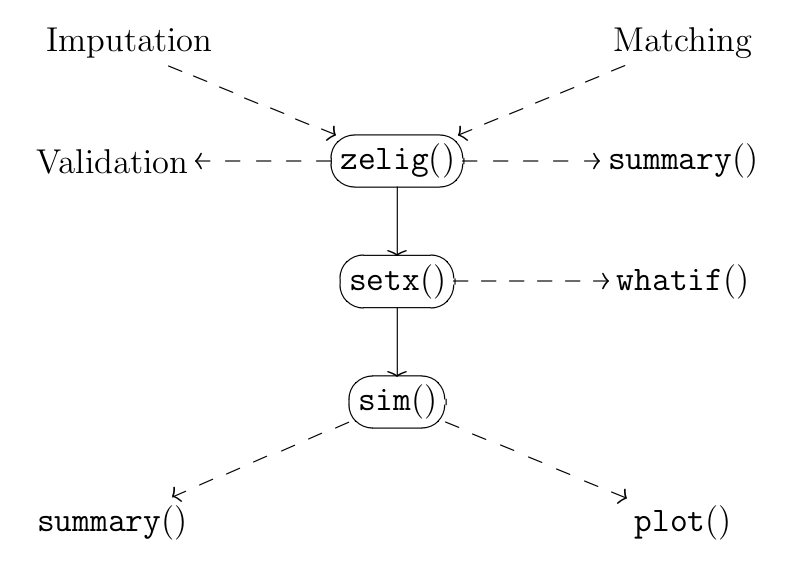
\includegraphics{main_commands.png}

1. Use \code{zelig()} to run the chosen statistical model on a given data set, with a specific
set of variables. For standard likelihood models, for example, this step estimates the
coefficients, other model parameters, and a variance-covariance matrix. In addition,
you may choose from a variety of options:
\begin{itemize}
\item {} 
Pre-process data: Prior to calling \code{zelig()}, you may choose from a variety of
data pre-processing commands (matching or multiple imputation, for example)
to make your statistical inferences more accurate.

\item {} 
Summarize model: After calling \code{zelig()}, you may summarize the fitted model
output using \code{summary()}.

\item {} 
Validate model: After calling \code{zelig()}, you may choose to validate the fitted model.
This can be done, for example, by using cross-validation procedures and diagnostics tools.

\end{itemize}

2. Use \code{setx()} to set each of the explanatory variables to chosen (actual or counterfactual)
values in preparation for calculating quantities of interest. After calling \code{setx()},
you may use \code{WhatIf} to evaluate these choices by determining whether they involve
interpolation (i.e., are inside the convex hull of the observed data) or extrapolation,
as well as how far these counterfactuals are from the data. Counterfactuals chosen in
\code{setx()} that involve extrapolation far from the data can generate considerably more
model dependence (see (37), (39), (48)).

3. Use \code{sim()} to draw simulations of your quantity of interest (such as a predicted value,
predicted probability, risk ratio, or first difference) from the model. (These simulations
may be drawn using an asymptotic normal approximation (the default), bootstrapping,
or other methods when available, such as directly from a Bayesian posterior.) After
calling \code{sim()}, use any of the following to summarize the simulations:
\begin{itemize}
\item {} 
The \code{summary()} function gives a numerical display. For multiple \code{setx()} values,
\code{summary()} lets you summarize simulations by choosing one or a subset of observations.

\item {} 
If the \code{setx()} values consist of only one observation, \code{plot()} produces density
plots for each quantity of interest.

\end{itemize}

Whenever possible, we use \code{z.out} as the \code{zelig()} output object, \code{x.out} as the \code{setx()} output
object, and \code{s.out} as the \code{sim()} output object, but you may choose other names.


\subsection{Examples}
\label{4_statistical_commands:examples}\begin{itemize}
\item {} 
Use the turnout data set included with Zelig to estimate a logit model of an individual’s
probability of voting as function of race and age. Simulate the predicted probability of
voting for a white individual, with age held at its mean:

\end{itemize}

\begin{Verbatim}[commandchars=\\\{\}]
data\PYG{p}{(}turnout\PYG{p}{)}
z.out \PYG{o}{\PYGZlt{}\PYGZhy{}} zelig\PYG{p}{(}vote \PYG{o}{\PYGZti{}} race \PYG{o}{+} age\PYG{p}{,} model \PYG{o}{=} \PYG{l+s}{\PYGZdq{}}\PYG{l+s}{logit\PYGZdq{}}\PYG{p}{,} data \PYG{o}{=} turnout\PYG{p}{)}
x.out \PYG{o}{\PYGZlt{}\PYGZhy{}} setx\PYG{p}{(}z.out\PYG{p}{,} race \PYG{o}{=} \PYG{l+s}{\PYGZdq{}}\PYG{l+s}{white\PYGZdq{}}\PYG{p}{)}
s.out \PYG{o}{\PYGZlt{}\PYGZhy{}} sim\PYG{p}{(}z.out\PYG{p}{,} x \PYG{o}{=} x.out\PYG{p}{)}
summary\PYG{p}{(}s.out\PYG{p}{)}
\end{Verbatim}
\begin{itemize}
\item {} 
Compute a first difference and risk ratio, changing education from 12 to 16 years, with
other variables held at their means in the data:

\end{itemize}

\begin{Verbatim}[commandchars=\\\{\}]
data\PYG{p}{(}turnout\PYG{p}{)}
z.out \PYG{o}{\PYGZlt{}\PYGZhy{}} zelig\PYG{p}{(}vote \PYG{o}{\PYGZti{}} race \PYG{o}{+} educate\PYG{p}{,} model \PYG{o}{=} \PYG{l+s}{\PYGZdq{}}\PYG{l+s}{logit\PYGZdq{}}\PYG{p}{,} data \PYG{o}{=} turnout\PYG{p}{)}
x.low \PYG{o}{\PYGZlt{}\PYGZhy{}} setx\PYG{p}{(}z.out\PYG{p}{,} educate \PYG{o}{=} \PYG{l+m}{12}\PYG{p}{)}
x.high \PYG{o}{\PYGZlt{}\PYGZhy{}} setx\PYG{p}{(}z.out\PYG{p}{,} educate \PYG{o}{=} \PYG{l+m}{16}\PYG{p}{)}
s.out \PYG{o}{\PYGZlt{}\PYGZhy{}} sim\PYG{p}{(}z.out\PYG{p}{,} x \PYG{o}{=} x.low\PYG{p}{,} x1 \PYG{o}{=} x.high\PYG{p}{)}
summary\PYG{p}{(}s.out\PYG{p}{)}
\PYG{c+c1}{\PYGZsh{} Numerical summary.}
plot\PYG{p}{(}s.out\PYG{p}{)}
\end{Verbatim}
\begin{itemize}
\item {} 
Calculate expected values for every observation in your data set:

\end{itemize}

\begin{Verbatim}[commandchars=\\\{\}]
data\PYG{p}{(}turnout\PYG{p}{)}
z.out \PYG{o}{\PYGZlt{}\PYGZhy{}} zelig\PYG{p}{(}vote \PYG{o}{\PYGZti{}} race \PYG{o}{+} educate\PYG{p}{,} model \PYG{o}{=} \PYG{l+s}{\PYGZdq{}}\PYG{l+s}{logit\PYGZdq{}}\PYG{p}{,} data \PYG{o}{=} turnout\PYG{p}{)}
x.out \PYG{o}{\PYGZlt{}\PYGZhy{}} setx\PYG{p}{(}z.out\PYG{p}{,} fn \PYG{o}{=} \PYG{k+kc}{NULL}\PYG{p}{)}
s.out \PYG{o}{\PYGZlt{}\PYGZhy{}} sim\PYG{p}{(}z.out\PYG{p}{,} x \PYG{o}{=} x.out\PYG{p}{)}
summary\PYG{p}{(}s.out\PYG{p}{)}
\end{Verbatim}
\begin{itemize}
\item {} 
Use five multiply imputed data sets from (47) in an ordered logit model:

\end{itemize}

\begin{Verbatim}[commandchars=\\\{\}]
data\PYG{p}{(}immi1\PYG{p}{,} immi2\PYG{p}{,} immi3\PYG{p}{,} immi4\PYG{p}{,} immi5\PYG{p}{)}
z.out \PYG{o}{\PYGZlt{}\PYGZhy{}} zelig\PYG{p}{(}as.factor\PYG{p}{(}ipip\PYG{p}{)} \PYG{o}{\PYGZti{}} wage1992 \PYG{o}{+} prtyid \PYG{o}{+} ideol\PYG{p}{,} model \PYG{o}{=} \PYG{l+s}{\PYGZdq{}}\PYG{l+s}{ologit\PYGZdq{}}\PYG{p}{,}
    data \PYG{o}{=} mi\PYG{p}{(}immi1\PYG{p}{,} immi2\PYG{p}{,} immi3\PYG{p}{,} immi4\PYG{p}{,} immi5\PYG{p}{)}\PYG{p}{)}
\end{Verbatim}
\begin{itemize}
\item {} 
Use the nearest propensity score matching via MatchIt package, and then calculate the
conditional average treatment effect of the job training program based on the linear
regression model:

\end{itemize}

\begin{Verbatim}[commandchars=\\\{\}]
library\PYG{p}{(}MatchIt\PYG{p}{)}
data\PYG{p}{(}lalonde\PYG{p}{)}
m.out \PYG{o}{\PYGZlt{}\PYGZhy{}} matchit\PYG{p}{(}treat \PYG{o}{\PYGZti{}} re74 \PYG{o}{+} re75 \PYG{o}{+} educ \PYG{o}{+} black \PYG{o}{+} hispan \PYG{o}{+} age\PYG{p}{,} data \PYG{o}{=} lalonde\PYG{p}{,}
    method \PYG{o}{=} \PYG{l+s}{\PYGZdq{}}\PYG{l+s}{nearest\PYGZdq{}}\PYG{p}{)}
m.data \PYG{o}{\PYGZlt{}\PYGZhy{}} match.data\PYG{p}{(}m.out\PYG{p}{)}
z.out \PYG{o}{\PYGZlt{}\PYGZhy{}} zelig\PYG{p}{(}re78 \PYG{o}{\PYGZti{}} treat \PYG{o}{+} distance \PYG{o}{+} re74 \PYG{o}{+} re75 \PYG{o}{+} educ \PYG{o}{+} black \PYG{o}{+} hispan \PYG{o}{+}
    age\PYG{p}{,} data \PYG{o}{=} m.data\PYG{p}{,} model \PYG{o}{=} \PYG{l+s}{\PYGZdq{}}\PYG{l+s}{ls\PYGZdq{}}\PYG{p}{)}
x.out0 \PYG{o}{\PYGZlt{}\PYGZhy{}} setx\PYG{p}{(}z.out\PYG{p}{,} fn \PYG{o}{=} \PYG{k+kc}{NULL}\PYG{p}{,} treat \PYG{o}{=} \PYG{l+m}{0}\PYG{p}{)}
x.out1 \PYG{o}{\PYGZlt{}\PYGZhy{}} setx\PYG{p}{(}z.out\PYG{p}{,} fn \PYG{o}{=} \PYG{k+kc}{NULL}\PYG{p}{,} treat \PYG{o}{=} \PYG{l+m}{1}\PYG{p}{)}
s.out \PYG{o}{\PYGZlt{}\PYGZhy{}} sim\PYG{p}{(}z.out\PYG{p}{,} x \PYG{o}{=} x.out0\PYG{p}{,} x1 \PYG{o}{=} x.out1\PYG{p}{)}
summary\PYG{p}{(}s.out\PYG{p}{)}
\end{Verbatim}
\begin{itemize}
\item {} 
Validate the fitted model using the leave-one-out cross validation procedure and calculating
the average squared prediction error via \code{boot} package. For example:

\end{itemize}

\begin{Verbatim}[commandchars=\\\{\}]
library\PYG{p}{(}boot\PYG{p}{)}
data\PYG{p}{(}turnout\PYG{p}{)}
z.out \PYG{o}{\PYGZlt{}\PYGZhy{}} zelig\PYG{p}{(}vote \PYG{o}{\PYGZti{}} race \PYG{o}{+} educate\PYG{p}{,} model \PYG{o}{=} \PYG{l+s}{\PYGZdq{}}\PYG{l+s}{logit\PYGZdq{}}\PYG{p}{,} data \PYG{o}{=} turnout\PYG{p}{,} cite \PYG{o}{=} \PYG{k+kVariable}{F}\PYG{p}{)}
cv.out \PYG{o}{\PYGZlt{}\PYGZhy{}} cv.glm\PYG{p}{(}z.out\PYG{p}{,} data \PYG{o}{=} turnout\PYG{p}{,} k \PYG{o}{=} \PYG{l+m}{11}\PYG{p}{)}
print\PYG{p}{(}cv.out\PYG{o}{\PYGZdl{}}delta\PYG{p}{)}
\end{Verbatim}


\subsection{Details}
\label{4_statistical_commands:details}\begin{enumerate}
\item {} 
\code{z.out \textless{}- zelig(formula, model, data, by = NULL, ...)}

\end{enumerate}

The \code{zelig()} command estimates a selected statistical model given the specified data.
You may name the output object (\code{z.out} above) anything you desire. You must include
three required arguments, in the following order:
\begin{enumerate}
\item {} 
\code{formula} takes the form \code{y \textasciitilde{} x1 + x2}, where \code{y} is the dependent variable and \code{x1}
and \code{x2} are the explanatory variables, and \code{y}, \code{x1}, and \code{x2} are contained in the
same dataset. The \code{+} symbol means “inclusion” not “addition.” You may include
interaction terms in the form of \code{x1*x2} without having to compute them in prior
steps or include the main effects separately. For example, R treats the formula \code{y
\textasciitilde{} x1*x2} as \code{y \textasciitilde{} x1 + x2 + x1*x2}. To prevent R from automatically including
the separate main effect terms, use the \code{I()} function, thus: \code{y \textasciitilde{} I(x1 * x2)}.

\item {} 
\code{model} lets you choose which statistical model to run. You must put the name
of the model in quotation marks, in the form \code{model = "ls"}, for example. See
Section ??4.3?? for a list of currently supported models.

\item {} 
\code{data} specifies the data frame containing the variables called in the formula, in the
form \code{data = mydata}. Alternatively, you may input multiply imputed datasets in
the form \code{data = mi(data1, data2, ...)}. \footnote{
Multiple imputation is a method of dealing with missing values in your data which is more powerful
than the usual list-wise deletion approach. You can create multiply imputed datasets with a program such
as Amelia; see King, Honaker, Joseph, Scheve (2000).
} If you are working with matched
data created using \code{MatchIt}, you may create a data frame within the \code{zelig()}
statement by using \code{data = match.data(...)}. In all cases, the data frame or
MatchIt object must have been previously loaded into the working memory.

\item {} 
\code{by} (an optional argument which is by default \code{NULL}) allows you to choose a factor
variable (see Section ??2??) in the data frame as a subsetting variable. For each of
the unique strata defined in the by variable, \code{zelig()} does a separate run of the
specified model. The variable chosen should not be in the formula, because there
will be no variance in the by variable in the subsets. If you have one data set for
all 191 countries in the UN, for example, you may use the by option to run the
same model 191 times, once on each country, all with a single \code{zelig()} statement.
You may also use the \code{by} option to run models on \code{MatchIt} subclasses.

\item {} 
The output object, \code{z.out}, contains all of the options chosen, including the name of
the data set. Because data sets may be large, Zelig does not store the full data set,
but only the name of the dataset. Every time you use a Zelig function, it looks for
the dataset with the appropriate name in working memory. (Thus, it is critical
that you do not change the name of your data set, or perform any additional
operations on your selected variables between calling \code{zelig()} and \code{setx()}, or
between \code{setx()} and \code{sim()}.)

\item {} 
If you would like to view the regression output at this intermediate step, type
\code{summary(z.out)} to return the coefficients, standard errors, t-statistics and p-
values. We recommend instead that you calculate quantities of interest; creating
\code{z.out} is only the first of three steps in this task.

\end{enumerate}
\begin{enumerate}
\setcounter{enumi}{1}
\item {} 
\code{x.out \textless{}- setx(z.out, fn = list(numeric = mean, ordered = median, others = mode), data = NULL, cond = FALSE, ...)}

\end{enumerate}
\begin{quote}

The \code{setx()} command lets you choose values for the explanatory variables, with which
\code{sim()} will simulate quantities of interest. There are two types of \code{setx()} procedures:
\begin{quote}
\begin{itemize}
\item {} 
You may perform the usual unconditional prediction (by default, \code{cond = FALSE}),

\end{itemize}
\begin{quote}

by explicitly choosing the values of each explanatory variable yourself or letting
\code{setx()} compute them, either from the data used to create \code{z.out} or from a new
data set specified in the optional data argument. You may also compute predictions
for all observed values of your explanatory variables using \code{fn = NULL}.
\end{quote}
\end{quote}
\begin{itemize}
\item {} 
Alternatively, for advanced uses, you may perform conditional prediction (\code{cond = TRUE}),

\end{itemize}
\begin{quote}

which predicts certain quantities of interest by conditioning on the observed value of the dependent variable.
In a simple linear regression model, this
procedure is not particularly interesting, since the conditional prediction is merely
the observed value of the dependent variable for that observation. However, conditional prediction
is extremely useful for other models and methods, including
the following:
\begin{itemize}
\item {} 
In a matched sampling design, the sample average treatment effect for the
treated can be estimated by computing the difference between the observed
dependent variable for the treated group and their expected or predicted
values of the dependent variable under no treatment (16).

\item {} 
With censored data, conditional prediction will ensure that all predicted values
are greater than the censored observed values (28).

\item {} 
In ecological inference models, conditional prediction guarantees that the predicted values are on the tomography line and
thus{}`{}`.

\end{itemize}
\end{quote}
\end{quote}


\chapter{Indices and tables}
\label{index:indices-and-tables}\begin{itemize}
\item {} 
\emph{genindex}

\item {} 
\emph{modindex}

\item {} 
\emph{search}

\end{itemize}



\renewcommand{\indexname}{Index}
\printindex
\end{document}
